\documentclass{article}
\usepackage[spanish]{babel}

% Set page size and margins
% Replace `letterpaper' with`a4paper' for UK/EU standard size
\usepackage[a4paper,top=2cm,bottom=2cm,left=2cm,right=2cm,marginparwidth=2cm]{geometry}

\usepackage{amsmath}
\usepackage{graphicx}
\usepackage{amsfonts}
\usepackage{amssymb}
\usepackage[colorlinks=true, allcolors=blue]{hyperref}
\title{\textbf{MÁSTER UNIVERSITARIO EN
LÓGICA, COMPUTACIÓN E INTELIGENCIA ARTIFICIAL}}
\date{}
\begin{document}

\maketitle
\begin{flushleft}
\textbf{Aprendizaje Automático}
\\\textbf{Apellidos:} Lorenz Vieta
\\\textbf{Nombre:} Germán
\end{flushleft}


\section*{Cuestión 1}
¿Cuantas posibles hipótesis podemos representar mediante árboles de decisión si tenemos n atributos binarios?.\\

Supongamos que tenemos \(n\) atributos booleanos, tendremos entonces \(2^n\) posibles combinaciones.
Por otro lado como las hipótesis son funciones del tipo \(h :\Rightarrow \{0,1\}\). Entonces, habrá \(2^{2n}\)
posibles hipótesis para un árbol binario de \(n\) atributos.


\section*{Cuestión 2}
Definimos el tamaño de un árbol como el número de sus nodos, incluida las hojas. Dar dos árboles de tamaño distinto que representen la misma hipótesis.\\\\

Por ejemplo, si consideramos  un árbol  con nodo Mascota y hojas Perro y Gato, este árbol seria de tamaño 1 y representaría a siguiente hipótesis: \((perro,1,Pos)\).\\\\
\begin{center}
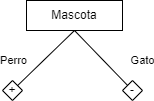
\includegraphics[scale=0.5]{mascota_1.png}\end{center}\\
Luego si consideramos otro árbol donde la hoja Gato lleva a un Nodo Raza con hojas Bengala y Siamés este árbol tendría tamaño 2 y también representaría la hipótesis \((perro,1,Pos)\).\\\\
\begin{center}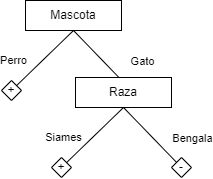
\includegraphics[scale=0.5]{mascota_2.png}\end{center}\\


\section*{Cuestión 3}
Dado el conjunto de entrenamiento y como conjunto de hipótesis H el conjunto de todos los árboles de decisión, dar dos elementos del espacio de versiones \(VS\). Uno de ellos debe clasificar de manera positiva y
otro de manera negativa el ejemplo
\begin{table}[!htbp]
\begin{align*}
    \begin{tabular}{|lllllll|}
    \hline
    Cielo   & Temperatura & Humedad & Viento & Agua     & Previsión & Deporte \\ \hline
    Soleado & Templada    & Normal  & Fuerte & Templada & Igual     & Sí      \\
    Soleado & Templada    & Alta    & Fuerte & Templada & Igual     & Sí      \\
    Lluvia  & Fría        & Alta    & Fuerte & Templada & Cambio    & No      \\
    Soleado & Templada    & Alta    & Fuerte & Fría     & Cambio    & Sí      \\ \hline
    \end{tabular}
\end{align*}
\end{table}
\begin{center}\(\langle Lluvia, Templada, Normal, Fuerte, Templada, Cambio \rangle\)\end{center}
Podemos considerar el siguiente árbol de decisión. Este árbol clasifica de manera negativa al ejemplo:
\begin{center}\(\langle Lluvia, Templada, Normal, Fuerte, Templada, Cambio \rangle\)\\\\
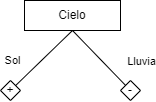
\includegraphics[scale=0.5]{tiempo_1.png}\end{center}\\
Por otro lado esté árbol clasifica correctamente y de manera positiva el ejemplo\\
\begin{center}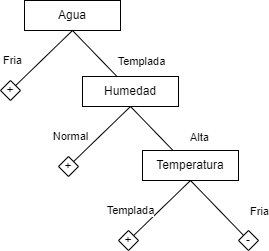
\includegraphics[scale=0.5]{tiempo_2.png}\end{center}\\

\section*{Cuestión 4}
En un problema de aprendizaje sobre el que vamos a aplicar el algoritmo ID3 se considera un conjunto de entrenamiento $D$ con $N$ ejemplos. Supongamos que hay un atributo $Atr_1$ que puede tomar $N$ valores y que cada uno de los ejemplos de $D$ toma en $Atr_1$ un valor distinto. Calcular \emph{Ganancia}($D$, $Atr_1$).\\
\[Ganancia(D, Atr_1)={Ent}(D)-
\sum_{v \in valores Atr_1 }=\frac{|D_v|}{|D|}{Ent}(D_v)\]\\
Sea \(v \in Valores(Atr_1)\), entonces \(|D_v| = 1, |D| = N\).\\\\
Además, \(Ent(D_v) =
\left\{
	\begin{array}{ll}
	    Ent([1^+,0^-]) = 0 & \mbox{si } D_v Pos  \\
		Ent([0^-,1^+]) = 0 & \mbox{si } D_v Neg
	\end{array}
\right.\)\\\\
Luego el segundo miembro de la ${Ganancia}(D, Atr_1)$ es la suma de tantos ceros como valores
tenga el atributo $Atr_1$. Por tanto:
\begin{center}$Ganancia(D; Atr1) = Ent(D)$\end{center}\\

\section*{Cuestión 5}
Demostrar que si $D$ es un conjunto de entrenamiento para un concepto $C$ entonces el algoritmo ID3 devuelve una hipótesis consistente con $D$ cualquiera que sea el criterio para elegir el \emph{mejor} atributo\\\\

Por reducción al absurdo, tenemos un nuevo algoritmo ID3 que devuelve en el Paso 4 un atributo $A$ y este da lugar a una hipótesis $h$ no consistente con $D$, osea, existe un ejemplo \(E \in D\) para el que $h$ toma valor positivo cuando mi árbol predice el valor negativo, o viceversa. Por tanto, tenemos un atributo $X$ en el que se difiere.\\\\
Entonces, en algún momento en la construcción del árbol se debe haber elegido $X$ como el atributo que mejor clasifica, es decir, $X$ sigue el algoritmo nuevo ID3 y es acorde a todos los ejemplos de $D$, incluido $E$.\\\\
Si esto es posible, entonces esto es una contradicción, luego $h$ es consistente y por tanto la elección de $A$ da lugar a una hipótesis consistente sea cual sea el criterio que se ha usado para elegir el mejor atributo.\\

\section*{Cuestión 6}
Sea $U$ un universo finito y sea $C$ un concepto sobre $U$ donde las instancias se representan como $n$-uplas de pares atributo-valor. Entonces $C$ puede representarse como un árbol de decisión.\\

De forma genérica si un conjunto de entrenamiento $D$ esta formado por un conjunto de instancias de forma:
\begin{center}
\(x^i=(\langle Atr_1,Valor_1^i\rangle,\langle Atr_2,Valor_2^i\rangle, ... ,\langle Atr_{n-1},Valor_{n-1}^i\rangle,\langle Atr_n,Valor_n^i\rangle)\)
\end{center}
para las que se conoce el valor del concepto $C$,$c(x^i)$. Entonces se puede representar en una tabla con la forma:\\
\begin{align*}
\begin{tabular}{|c|c|c|c|c|c|c|}
\hline
\textit{} & \textbf{$Atr_1$} & $Atr_2$  & ...  & $Atr_{n-1}$ & $Atr_{n}$ & Concepto   \\ \hline
$x^1$     & $Valor_1^1$     & $Valor_2^1$     & ... & $Valor_{n-1}^1$     & $Valor_{n}^1$     & $c(x^1)$\\ \hline
$x^2$     & $Valor_1^2$     & $Valor_2^2$     & ... & $Valor_{n-1}^2$     & $Valor_{n}^2$     & $c(x^2)$\\ \hline
...         & ...             & ...             & ... & ...                 & ...                & ...\\ \hline
$x^{i-1}$ & $Valor_1^{i-1}$ & $Valor_2^{i-1}$ & ... & $Valor_{n-1}^{i-1}$ & $Valor_{n}^{i-1}$ & $c(x^{i-1})$\\ \hline
$x^{i}$   & $Valor_1^{i}$   & $Valor_2^{i}$   & ... & $Valor_{n-1}^{i}$   & $Valor_{n}^{i}$   & $c(x^{i})$\\ \hline
\end{tabular}
\end{align*}
Podemos aplicar el algoritmo ID3 (Ejemplos, Atributo-Objetivo, Atributos) a la tabla anterior usando:
\begin{enumerate}
    \item Ejemplos: $x^i$
    \item Atributo-Objetivo: $c(x^{i})$
    \item  Atributo: $Atr_1, ..., Atr_n$
\end{enumerate}
De esa forma se representara como un árbol de decisión

\section*{Cuestión 7}
Responder razonadamente si las siguientes afirmaciones son verdaderas o falsas. Si la respuesta \textbf{Verdadera} debes dar razones que apoyen tu decisión. Si la respuesta es \textbf{Falsa} debes dar un ejemplo en el que no se verifique la afirmación.
\begin{enumerate}
    \item Sea $D_1 = \{e_1,..., e_n\}$ un conjunto de entrenamiento y sea $D_2$ el conjunto de entrenamiento formado a partir de $D_1$ donde cada ejemplo se considera dos veces, esto es, $D_2 = \{e_1,...,e_n,e_{n+1},...,e_{2n}\}$ donde $\forall i\in\{1,...,n\}e_i = e_{i+n}$. Afirmación: \emph{El árbol de decisión obtenido mediante el algoritmo ID3 a partir de $D_1$ y $D_2$ son el mismo}.\\
    
    \textbf{Verdadero}: Según Algoritmo ID3:\\\\
    \textbf{Paso 1}: Si todos los Ejemplos son positivos, devolver un nodo etiquetado con $+$.  Entonces si todos son positivos en $D_1$ lo van a ser en $D_2$.\\
    \textbf{Paso 2}: Si todos los Ejemplos son negativos, devolver un nodo etiquetado con $-$. Entonces si todos son negativos en $D_1$ lo van a ser en $D_2$.\\
    \textbf{Paso 3}: Si Atributos está vacío, devolver un nodo etiquetado con el valor más frecuente de Atributo-objetivo en Ejemplos. Entonces Si el valor más frecuente en Ejemplos de $D_1$ es el mismo que para $D_2$ y dará el mismo ejemplo.\\
    \textbf{Paso 4}: En otro caso:\\
    \textbf{Paso 4.1}: Sea A el atributo de Atributos que mejor clasifica hacer:
    \[Ganancia(D, Atr_1)={Ent}(D)-\sum_{v \in valores Atr_1 }=\frac{|D_v|}{|D|}{Ent}(D_v)\]
    Sean $P_1$, $N_1$ los positivos y negativos de $D_1$ entonces:\\\\
    \(Ent(D_1)=-\frac{|P_1|}{|D_1|}log_2\frac{|P_1|}{|D_1|}-\frac{|N_1|}{|D_1|}log_2\frac{|P_1|}{|D_1|}\)\\\\
    \(Ent(D_2)=-\frac{|2P_1|}{|2D_1|}log_2\frac{|2P_1|}{|2D_1|}-\frac{|2N_1|}{|2D_1|}log_2\frac{|2P_1|}{|2D_1|}=Ent(D_1)\)\\\\
    Igualmente, $Ent(D{1v})=Ent(D{2v})$, por lo tanto el atributo sera el mismo.\\\\
    \textbf{Paso 4.2}: Crear Árbol, con un nodo etiquetado con A, entonces sera igual en ambos casos\\
    \textbf{Paso 4.3}: Para cada posible valor $v$ de $A$, hacer:
    \begin{itemize}
    \item Añadir un arco al Árbol, etiquetado con $v$.
    \item Sea Ejemplos$(v)$ el subconjunto de Ejemplos con valor del atributo $A$ igual a $v$.
    \item Si Ejemplos$(v)$ es vacío:
        \begin{itemize}
        \item Entonces colocar debajo del arco anterior un nodo etiquetado con el valor más frecuente de Atributo-objetivo en Ejemplos.
        \end{itemize}
        \begin{itemize}
        \item Si no, colocar debajo del arco anterior el subárbol ID3 $(Ejemplos(v), Atributo-objetivo,
Atributos-A)$
        \end{itemize}
    De esta forma, si Ejemplos $(v)$ es vacío en $D_1$ lo va a ser también en $D_2$. De la misma forma, el valor más frecuente será el mismo en ambos árboles. Si no, repetimos el proceso para ID3 $(Ejemplos(v), Atributo-objetivo,Atributos-A)$ en los dos conjuntos de entrenamiento.\\\\
    Por lo tanto para los dos conjuntos de entrenamiento obtendremos el mismo árbol
    \end{itemize}
    \item Tenemos un conjunto con $4n$ ejemplos y lo dividimos en dos partes: un conjunto de entrenamiento con $3n$ ejemplos y un conjunto de prueba con $n$ ejemplos. En el conjunto de entrenamiento $2n$ ejemplos son positivos y $n$ ejemplos son negativos. En el conjunto de prueba, los $n$ ejemplos que hay son todos positivos. Construimos el árbol de decisión A a partir del conjunto de entrenamiento mediante el algoritmo ID3. Afirmación: \emph{El árbol A contiene al menos un nodo tal que si podamos en ese nodo mejoramos el rendimiento respecto al conjunto de prueba.}\\\\
    \textbf{Falso}: Si el árbol obtenido ya es óptimo en rendimiento en los casos de prueba al aplicar el algoritmo ID3 puede que obtengamos un árbol nuevo pero para los casos de prueba sera el mismo recorrido. Por lo tanto, existe la posibilidad de que la medida de casos correctamente clasificados positivamente sea 1 y el rendimiento de mi árbol mejorado con ID3 sea 1 demostrando que no hubo una mejora significativa al podarlo.\\
    Por ultimo, esta situación es poco probable en casos reales donde $n$ es un valor muy elevado.
    \item Sean $D_1$ y $D_2$ dos conjuntos de entrenamiento para el mismo concepto. Entonces
    \begin{align}
        \frac{Ent(D_1)+Ent(D_2)}{2}\le Ent(D_1\cup D_2)
    \end{align}
    \begin{itemize}
    \item  Si consideramos por ejemplo $D_1 = [4^+,4^-]$, $D_2 = [1^+,1^-]$ y $D_1 \cup D_2 = [5^+,5^-]$ entonces:\\\\
    $Ent(D_1)=1$, $Ent(D_2)=1$ y $Ent(D_1 \cup D_2)= 1$\\\\
    $\frac{Ent(D_1)+Ent(D_2)}{2} = \frac{2}{2}= 1 \leq 1 = Ent(D_1\cup D_2)$
    \item Si consideramos por ejemplo $D_1 = [0^+,34^-]$, $D_2 = [1^+,1^-]$ y $D_1 \cup D_2 = [1^+,35^-]$ entonces:\\\\
    $Ent(D_1)=0$, $Ent(D_2)=1$ y $Ent(D_1 \cup D_2)= -\frac{1}{35}log_2\frac{1}{35}-\frac{34}{35}log_2\frac{34}{35}\simeq0.18717$\\\\
    $\frac{Ent(D_1)+Ent(D_2)}{2} = \frac{1}{2} = 0.5 \nleq 0.18717 \simeq Ent(D_1\cup D_2)$
    \end{itemize}
    
    \textbf{Falso}: Al encontrar un contraejemplo no es valida la propiedad
    
    \item Sean $D_1$ y $D_2$ dos conjuntos de entrenamiento para el mismo concepto tales que $D_1 \cap D_2 \not = \emptyset$. Entonces $Ent(D_1 \cup D_2) < Ent(D_1) + Ent(D_2)$.\\
    
    Consideremos la siguiente tabla de ejemplos:
    \begin{flushleft}
    \begin{tabular}{||c | c ||}
    \hline
    Color    & Clasificación de semáforo peatonal\\ \hline
    Verde    & Positivo \\ 
    Rojo     & Negativo \\ \hline
    \end{tabular}
    \end{flushleft}\\
    Consideremos $D_1$ como la primer fila y $D_2$ la segunda, tenemos entonces que $Ent(D_1)=Ent(D_2) = 0$.\\
    Además, $D_1 \cup D_2$ será la tabla completa y como $Ent(D_1 \cup D_2) = Ent([1^+, 1^-]) = 1$\\
    Entonces, encontramos que $Ent(D_1 \cup D_2) = 1 \nless 0 = Ent(D_1) + Ent(D_2)$\\\\
    \textbf{Falso}: Al encontrar un contraejemplo no es valida la propiedad
    \end{enumerate}


\section*{Cuestión 8}
La ganancia de información en el algoritmo ID3 sólo sirve para hacer árboles más pequeños. Si aplicamos el algoritmo de árboles de decisión sobre un mismo conjunto de entrenamiento dos veces, la primera utilizando la ganancia de información para elegir el mejor atributo y la segunda vez utilizando otro criterio, entonces los dos árboles obtenidos pueden tener distinto tamaño, pero representan la misma hipótesis. \textbf{¿Verdadero o falso?}\\

\textbf{Falso}: Es verdadero que la ganancia de información en el algoritmo ID3 sirve para encontrar atributos más representativos y que ayudan a clasificar mejor los ejemplos y con esto puede existir la posibilidad de reducción del tamaño del árbol, pero esto no implica que la aplicación de ID3 vaya a devolvernos un árbol de igual tamaño que con otros métodos o criterios.\\
También es cierto que aplicando distintos métodos se pueden obtener arboles de distinto tamaño que representan la misma hipótesis, pero nada nos asegura que otros algoritmos distintos a ID3 generen arboles del mismo tamaño y a la vez representen la misma hipótesis.

\section*{Ejercicio 1}
Supongamos que hemos dividido un conjunto de 25 ejemplos en dos conjuntos. El primero $D$ con 20 ejemplos lo hemos usado para crear un árbol de decisión y el segundo \emph{Prueba}, con 5 ejemplos, los vamos a usar para aplicar el \textsc{Algoritmo de poda para reducir el error}. El árbol obtenido y el conjunto de prueba son los siguientes:\\

{\centering
\begin{minipage}{0.45\textwidth}
   \centering
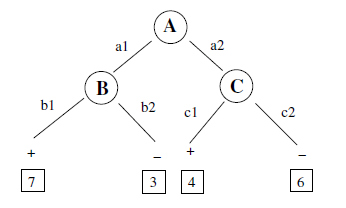
\includegraphics[width=60mm]{arbol_1.png}
\end{minipage}
\begin{minipage}{0.45\textwidth}
   \centering
\begin{tabular}{|c|c|c|c|c|}
\hline
\textit{} & \textbf{A} & B  & C  & Cl. \\ \hline
$e_1$      & a1         & b1 & c1 & +   \\ \hline
$e_2$      & a2         & b1 & c2 & +   \\ \hline
$e_3$      & a1         & b2 & c1 & +   \\ \hline
$e_4$      & a1         & b2 & c2 & +   \\ \hline
$e_5$      & a2         & b2 & c1 & +   \\ \hline
\end{tabular}
\end{minipage}
}
\begin{flushleft}
Junto a la clasificación de cada hoja aparece el número de elementos del conjunto $D$ que verifica la condición, esto es, hay 7 ejemplos con A=a1 y B=b1 que tienen clasificación $+$, hay 3 ejemplos con A=a1 y B=b2 que tienen clasificación $-$, etc. Se pide usar el \textsc{Algoritmo de poda para reducir el error} sobre el árbol usando el conjunto \emph{Prueba}. \textbf{Especificar claramente cuál es el árbol obtenido}.
\end{flushleft}
Primero: Calculamos la medida del arbol $M$ con los ejemplos:
\begin{itemize}
    \item $e_1$: Clasificación: $+$, Valor real $+$
    \item $e_2$: Clasificación: $-$, Valor real $+$
    \item $e_3$: Clasificación: $-$, Valor real $+$
    \item $e_4$: Clasificación: $-$, Valor real $+$
    \item $e_5$: Clasificación: $+$, Valor real $+$
\end{itemize}
Por tanto, $M = 2/5 = 0,4$\\\\
Ahora aplicamos el \textsc{Algoritmo de poda} por cada nodo y calculamos su medida correspondiente:\\
\begin{itemize}
    \item Podamos B, como hay 7 ejemplos $+$ y 3 $-$, se le asigna el valor $+$ a la rama libre al podar B y de esta forma se obtiene:
    \begin{itemize}
        \item $e_1$: Clasificación: $+$, Valor real $+$
        \item $e_2$: Clasificación: $-$, Valor real $+$
        \item $e_3$: Clasificación: $+$, Valor real $+$
        \item $e_4$: Clasificación: $+$, Valor real $+$
        \item $e_5$: Clasificación: $+$, Valor real $+$
    \end{itemize}
    Por tanto, $M_B = 4/5 = 0,8$
    \item Podamos C, como hay 4 ejemplos $+$ y 6 $-$, se le asigna el valor $-$ a la rama libre al podar C y de esta forma se obtiene:
    \begin{itemize}
        \item $e_1$: Clasificación: $+$, Valor real $+$
        \item $e_2$: Clasificación: $-$, Valor real $+$
        \item $e_3$: Clasificación: $-$, Valor real $+$
        \item $e_4$: Clasificación: $-$, Valor real $+$
        \item $e_5$: Clasificación: $-$, Valor real $+$
    \end{itemize}
    Por tanto, $M_C = 1/5 = 0,2$\\\\
    Termino los Nodo Hoja, comparo $K$ medias donde: $M_B>M_C$ y además $M_B > M$, entonces podo y devuelvo árbol resultante:
    \begin{center}
        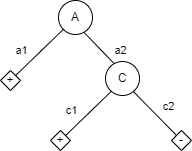
\includegraphics[scale=0.5]{arbol_2.png}
    \end{center}\\
\end{itemize}
\hline
\section*{Ejercicio opcional}
Demostrar que la ganancia de información es siempre mayor o igual a cero.
\end{document}